\clearpage

\def\chaptertitle{Range Thresholding on Streams}

\lhead{\emph{\chaptertitle}}

\chapter{\chaptertitle}
\label{ch:rts}

\section{Problem Definition}
\label{sec:rts-definition}
We will now formally define the Range Threshold on Streams (RTS) problem. Given a constant integer $d\geq 1$, we consider the \textit{data space} $\mathbb{R}^d$. The \textit{data stream} is an unbounded sequence of elements where the $i$-th $(i\geq1)$ element is denoted as $e_i$ and is said to arrive a time $i$. Each element $e_i$ carries two static fields; $v(e_i)$ - a point in the data space and a weight $w(e_i)\in\mathbb{Z}$. An \textit{RTS query} $q$ specifies a $d$-dimensional axis-parallel rectangle $R_q$ and a given integer threshold $\tau_q$.

If the query is issued after receiving $e_j$ for some $j\geq 1$ then for $t\geq j+1$ we define $S(q,t)$ to represent the elements $e_{j+1},e_{j+2},\dots,e_t$ that \textit{stab} $R_q$. That is, 
$$S(q, t) := \{e_i | j < i \leq t \text{ and } e_i \in R_q\}$$
Define
$$W(q, t) := \sum_{e\in S(q,t)}w(e)$$
Then the \textit{maturity time} of a query $q$ is the smallest $t$ such that $W(q,t)\geq \tau_q$. For a steam of length $n$ (that is, the length of the stream at this point) we will abbrevaiate $S(q,n)$ as $S(q)$ and $W(q, n)$ as $W(q)$.

The RTS problem is to simultaneously support a set of $m$ RTS queries and to correctly report the maturity time of a each query. In addition to supporting a given set of RTS queries, a solution must also support the following two operations, Register$(q)$: accept a new query at the current moment (after the arrival of $e_n$) and Terminate$(q)$: stop a given query $q$.

\section{Benchmark Solutions}
\label{sec:benchmark-solutions}

The RTS problem is deceptively simple at first glance, given a new stream element $e$ we can check for each query $q$ whether $e \in R_q$ and then increment $W(q)$ accordingly. This algorithm is trivially correct, though results in a quadratic $\Theta(nm)$ computation. Whilst a quadratic runtime appears innocent, this method becomes intractable when $m$ is large. Our goal therefore, is to aim for subquadratic runtime.

We also emphasis that we are considering an \textit{unboundedly} long stream of elements, all solutions explored are restricted to have a memory footprint in terms of $m$, as a Data Structure on the data stream itself is guarnateed to become prohibitively large.

\subsection{Naive Algorithm}
\label{sec:naive-algorithm}

As a simple baseline approach we will formally outline the most naive algorithm for solving the RTS problem

\begin{algorithm}
\caption{Naive RTS}\label{alg:naive-rts}
\begin{algorithmic}[1]
\Procedure{Naive-RTS}{query set $Q^*$}
\State \text{for each $q\in Q^*$ initialise $c_q\gets 0$}
\For{ \text{each stream element $e$}}
\For{ \text{each $q\in Q^*$}}
\State \text{if $e\in R_q$ set $c_q \gets c_q + w(e)$}
\State \text{if $c_q \geq \tau_q$, mature query $q$}
\EndFor
\EndFor
\EndProcedure
\end{algorithmic}
\end{algorithm}

\subsection{Stabbing Data Structures}
\label{sec:stabbing-data-structs}

A well-studied type of query in the Computer Science literature is the so-called stabbing query

\begin{definition}[Stabbing Query] Given a point $v$ in the data space $\mathbb{R}^d$ report the set of intervals $I$ in some set $Q$ such that $v \in I$. The returned set of queries are set to \textit{stabbed} by $Q$.
\end{definition}

Clearly, the RTS problem defined in \cref{sec:rts-definition} is itself a generalised form of stabbing query. There are a number of data structures \cite{DBLP:conf/soda/Rahul15} that support Stabbing queries, which can naturally be applied in the context of the RTS problem. We consider some notable examples below. 

\textbf{Interval Trees.}

\textbf{R Trees.}

\section{DT Algorithm}
\label{sec:DT-algorithm}

As we have seen, all benchmark solutions are unable to escape the quadratic trap in runtime which become impractical for massive values in $m$ and $n$. In this section, we present the state of the art \textit{DT Algorithm} \cite{GAN16}, as well as prove its correctness and sub-quadratic runtime.

\subsection{Constrained RTS Case}
\label{ssec:constrained-DT-algorithm}

For the moment, we restrain the RTS problem in the following ways: Set the dimension of the data space $d = 1$ and assume for each stream element we have $w(e) =1$. Moreover, we enforce that all queries are registered at the beginning, before receiving the first stream element, and no query is allowed to be registered afterwards. We refer to this latter condition as the \textit{one-time registration constraint}.

We will now present and analyse a version of the DT Algorithm for solving this constrained problem, before extending the algorithm to solve the most general version of RTS problem given in \cref{sec:rts-definition}.

\textbf{The Endpoint Tree.} We begin by denoting $Q^*$ as the set of registered RTS queries. The first step of the algorithm is to construct a special binary tree $\mathcal{T}$ on the sorted endpoints of the intervals in $Q^*$. For the remainder of this thesis, any tree constructed this way will be reffered to as an \textit{endpoint tree}. For each vertex $v\in V(\mathcal{T})$ we define its \textit{jurisdiction interval} as follows: 

\begin{definition}[Jurisdiction Interval]
    For each $v\in V(\mathcal{T})$ the \textit{jurisdiction interval associated with v}, denoted by $I(v)$. When $v$ is a \textit{leaf node} of $\mathcal{T}$ then $I(v) := [x, x^\prime)$ where $x$ is the endpoint associated with $v$ and $x^\prime$ is the endpoint associated with the leaf succeeding $v$. In the case that $v$ is the rightmost leaf of $\mathcal{T}$ define $x^\prime = +\infty$. When $V$ is not a leaf, define $I(v) := I(v.left) \cup I(v.right)$ where \textit{v.left} and \textit{v.right} denote the left and right child nodes of $v$.
\end{definition} 

In addition to each vertex $v$ having a jurisdiction interval, we also initialise a \textit{count} for each vertex $c(v) \leftarrow 0$. Once the tree has been constructed we now commence the data stream. Let $e$ be an incoming stream element such that $v(e)$ is at least the leftmost endpoint of $\mathcal{T}$ (otherwise, $e$ can be safely ignored). Starting at the root, trace a path to a leaf of $\mathcal{T}$ based on which nodes $u\in V(\mathcal{T})$ satisfy $v(e) \in I(u)$. For each node $u$ that is traced we increment the corresponding counter $c(u) \leftarrow c(u) + 1$. We refer to this procedure as the \textit{element processing} portion of the algorithm and we prove the following claims: 

\begin{lemma} For any stream element $e$ and endpoint tree $\mathcal{T}$, $v(e)$ stabs at most one jurisdiction interval at each level of $\mathcal{T}$. That is, at each level of $\mathcal{T}$, there is precisely one node $u$ such that $v(e)\in I(u)$.
\end{lemma}
\begin{proof}
    By contradiction suppose that $v(e)$ stabs two intervals $I(u_1)$ and $I(u_2)$ at the same level. Then $I(u_1) \cap I(u_2)\neq \emptyset$ which means the right endpoint of $I(u_1)$ must be greater than the left endpoint of $I(u_2)$, which is not possible from the construction of the tree, as nodes where constructed based on sorted order.
\end{proof}

\begin{lemma} For a set of $m$ queries, an endpoint tree $\mathcal{T}$ can be constructed in $O(m\log m)$ time, and element processing requires $O(\log m)$ time for each stream element.
\end{lemma}
\begin{proof}
     $\mathcal{T}$ can be constructed by first sorting the $2m$ endpoints of the query set, then recursively constructing the tree based off of adjacent nodes in a \textit{bottom-up} manner. During the construction of the tree, each vertex's jursdiction interval and counter can be initialised in $O(1)$ time. The runtime is dominated by the sorting which is $O(2m \log 2m) = O(m\log m)$. As the binary tree is built in a \textit{bottom-up} approach, we are guaranteed that the resulting tree is height-balanced, which implies the height is $O(\log m)$. Using Lemma 3.2 we know that we must only consider a single node at level of $\mathcal{T}$, which implies the element processing cost is on the order of the height of the tree which is $O(\log m)$
\end{proof}

\begin{center}
\begin{figure}[h]
\centering
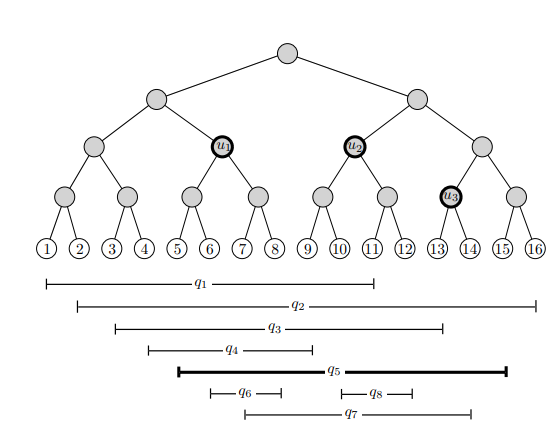
\includegraphics[scale=0.7]{thesis/figures/endpoint_tree.png}
\caption{An example of an endpoint tree with $I(u_3) = [13. 14)$, $I(u_2) = [9, 13)$ and $I(u_1) = [5, 9)$}
\end{figure}
\end{center}

\textbf{Applying Distributed Tracking.} We now reveal how nodes in the endpoint tree and their jurisdiction intervals coincide with RTS queries. Then, we will demonstrate how to effectively leverage Distributed Tracking algorithms to efficiently manage query maturation across the endpoint tree. First we require the following definition

\begin{definition}[Canoncial Node Set] For a given query $q\in Q^*$ with interval $R_q$ and endpoint tree $\mathcal{T}$ the \textit{Canonical node set} $U_q$ is the smallest $U_q\subseteq V(\mathcal{T})$ such that the jurisdiction intervals of $v\in U_q$ are pairwise disjoint and $R_q = \bigcup_{u\in U_q} I(u)$.
\end{definition}

For a given query $q$ with threshold $\tau_q$ and canonical node set $U_q$ we can consider a conceptual instance of distributed tracking with participants equal to $u_i\in U_q$, participant counters $c(u_i)$ as defined in the endpoint tree and coordinator threshold $\tau_q$. In this scenario, we view the query as the coordinator itself, whose mission is to capture the exact instant that 
\begin{equation}
    \tau_q = \sum_{u \in U_q} c(u) = W(q)
\end{equation}
We now execute an instance of \cref{alg:dist-tracking}, simulating each of its steps. We perform the element processing, and update each counter $c(u)$ in $\mathcal{T}$, these correspond to counter increments in \cref{alg:dist-tracking}. When condition $(3.1)$ is met via \cref{alg:dist-tracking}, this corresponds to query maturation in our range thresholding problem. 

As is emphasised in \cite{GAN16}, there is nothing \textit{distributed} in this configuration and all computation runs off of a single CPU. We simply leverage \cref{alg:dist-tracking} to efficiently identify the moment that an RTS query matures. To analyse the efficiency of the algorithm we will require the following lemmas:

\begin{lemma}
    For a given RTS query $q$ and endpoint tree $\mathcal{T}$, the canoncial node set $U_q$ can be determined in $O(\log m)$ time.
\end{lemma}
\begin{proof}
\end{proof}

\begin{lemma}
    For a given RTS query $q$ with canonical node set $U_q$ we have $|U_q| = O(\log m)$
\end{lemma}
\begin{proof}
\end{proof}

 As we have seen, each query $q\in Q^*$ defines an instance Distributed Tracking which we solve using \cref{alg:dist-tracking}. Recall from our description of \cref{alg:dist-tracking}, every node $u\in U_q$ maintains a counter $\Bar{c}_q(u)$ at the time of the last signal to the coordinator, $q$. The next signal from $u$ takes place 
\begin{equation}
    c(u) - \Bar{c}_q(u) = \lambda_q
\end{equation}
where $\lambda_q = \left\lfloor \frac{\tau_q}{2 |U|_q}\right\rfloor$ is the slack value described in \cref{alg:dist-tracking}. As part of the distributed tracking algorithm, the node $u$ needs to inspect condition (3.2) whenever $c(u)$ is incremented. By lemma 3.3 this implies $O(\log m)$ slack inspections per element processing. Theorem 2.5 gives the total messaging cost per query as $O(|U|_q\log \tau_q) = O(\log m\log\tau_q)$ by lemma 3.6.

\textbf{Organising Queries with Heaps.} The steps taken so far seem promising to result in a sub-quadratic algorithm, however let's pay close attention to the cost of inspecting the slack condition (3.2). For a given node $u\in V(\mathcal{T})$, let $Q(u)$ be the set set of queries that have $u$ in their canonical node set. Suppose that we have just incremented $c(u)$, if done naively, one would need to check condition $(3.2)$ for each $q\in Q(u)$. Clearly, this would require $O(|Q(u)|) = O(m)$ time, which coupled with $O(n\log m)$ element processing time for a stream of size $n$ would deprecate the performance of the algorithm to a quadratic $O(nm\log m)$.

Fortunately, with a few observations a we can leverage the Min-Heap described in \cref{sec:heap-data-structs} to avoid this. The idea is to inspect only \textit{one} slack condition in $Q(u)$, instead of all $|Q(u)|$. To see how one can do this, define for each $q$ the \textit{key}-value of 
\begin{equation}
    \sigma_q(u) := \lambda_q + \Bar{c}_q(u)
\end{equation}
where $\lambda_q, \Bar{c}_q$ correspond to values defined by \cref{alg:dist-tracking}. Intuitively $\sigma_q(u)$ represents the \textit{next} value of $c_q(u)$ for when the next signal from $u$ to coordinator $q$ should occur. The key observation is that, for $q_1, q_2 \in Q(u)$ with $\sigma_{q_{1}}(u) < \sigma_{q_{2}}(u)$ then $c_{q_1}(u) < c_{q_2}(u)$. That is, if we don't need to send a message for $q_1$, then we can immediately deduce that we do not need to send a messages for $q_2$. Using this key observation, we maintain a Min-Heap $\mathcal{H}(u)$ on $Q(u)$ for each $u\in V(\mathcal{T})$ and apply the following procedure whenever a counter is incremented.

\begin{algorithm}\label{alg:slack-inspection}
\begin{algorithmic}[1]
\Procedure{SlackInspection}{$u$}
\State \text{Find the minimum $\sigma_q(u)$ in $\mathcal{H}(u)$}
\State \text{If $\sigma_q(u) < c(u)$, then we are done.}
\State \text{Otherwise, remove $\sigma_q(u)$ from       
             $\mathcal{H}(u)$. }
\Statex \text{\hspace{5mm} Instruct $u$ to send a signal to $q$ as per \cref{alg:dist-tracking}}
\Statex \text{\hspace{5mm} \textbf{return} SlackInspection$(u)$}
\Comment{Recursive call}
\EndProcedure
\end{algorithmic}
\end{algorithm}

\textbf{Handling Matured Queries.} We now consider the space complexity of the DT algorithm.


\textbf{Analysis.} We have now motivated and explained each component of the DT algorithm. For the curious reader, we note that the algorithm is called \textit{DT} as a nod to it's use of \textit{Distributed Tracking}. We now prove correctness, and analyse the total complexity of the algorithm.

\begin{theorem}[Correctness] The Constrained DT algorithm solves the constrained RTS problem. That is, for each query $q$ the constrained DT algorithm correctly reports the instant that $W(q) = \tau_q$
\end{theorem}
\begin{proof}
    Each $q \in Q^*$ is mapped to an instance of Distributed Tracking which is then solved by \cref{alg:dist-tracking}. The correctness of reporting when $W(q) = \tau_q$ follows as a consequence of Theorem 2.5.
\end{proof}

\begin{theorem}[Time Complexity] For a collection of $m$ RTS queries and a stream of $n$ elements, the constrained DT algorithm requires $O(n\log m + m\log^2m\log\tau_{max})$ time.
\end{theorem}
\begin{proof}
\end{proof}

An important observation is that the runtime of the DT algorithm can be decomposed into the runtime of the \textit{element processing} (tracing a stream element through the endpoint tree) and the runtime of the \textit{communication cost} (the simulated messaging of \cref{alg:dist-tracking}). That is, 
$$O(\underbrace{n\log m}_{\text{element processing}} + \underbrace{m\log ^2 m\log\tau_{max}}_{\text{communication}})$$

For completeness, we completely describe the constrained DT algorithm in psuedocode below. 

\begin{algorithm}
\caption{Constrained DT}\label{alg:constrained-dt}
\begin{algorithmic}[1]
\Require $Q^* \gets m$ \text{ RTS queries $(R_q, \tau_q)$}
\State \text{Build end point tree $\mathcal{T}$ from endpoints in $Q^*$}
\For{ $q \in Q^*$}
    \State \text{Find canonical node set $U_q$}
    \State \text{Create instance of \cref{alg:dist-tracking} on $U_q$}
\EndFor
\State \text{Commence data stream} 
\For{$e_t$ for $t = 1,2,\dots$}
\State \text{Trace $e_t$ through $\mathcal{T}$ based on Jurisdiction Interval}
\State \text{Update node counters $c(v) \gets c(v)+1$ for each $v\in V(\mathcal{T})$ traced}
\State \text{Perform \cref{alg:slack-inspection} for each $v\in V(\mathcal{T})$ traced}
\EndFor
\end{algorithmic}
\end{algorithm}

\subsection{Unconstrained RTS Case}
\label{ssec:unconstrained-DT-algorithm}

We now reveal how \cref{alg:constrained-dt} can be extended to solve the full, unconstrained RTS problem. We will remove each constraint separately before revealing our complete algorithm. 

\textbf{Enabling Insertions.} The first constraint we will eliminate is the one-time registration condition; that is, will define how to incorporate a Register($q$) procedure for a new RTS query $q$. 

Our solution is to apply \textit{Logarithmic Rebuilding} described in \cref{sec:logarithmic-rebuilding}. The query set $Q^*$ is now partitioned into sets $S_1,\dots, S_h$ such that $h = O(\log m)$, each query set $S_i$ contains either $2^i$ queries, or is empty and importantly, each query belongs to precisely one $S_i$. Associated to each query set is an independent end-point tree $\mathcal{T}_1\dots, \mathcal{T}_h$, built on the endpoints of queries in $S_1,\dots,S_h$. Registering a new query is as described in \cref{sec:logarithmic-rebuilding}, identify the smallest $j$ such that $S_j = \emptyset$ and set $S_j = \bigcup_{i=1}^{j-1}S_i$ along with the new query $q$, and then create a new endpoint tree $\mathcal{T}$ on $S_j$.


To preserve the correctness of our original algorithm, given an incoming element $e$ we must now trace it through each $\mathcal{T}_1,\dots,\mathcal{T}_h$. As $h = O(\log m)$ and the height of each tree is $O(\log m)$ this implies an element processing cost of $O(n\log ^2 m)$ for a stream of length $n$.

\textbf{Multidimensional Queries.} 

\textbf{Weighted Stream Elements.} The final constraint to remove is the restriction of stream weights to be just 1. To achieve this, we will require a more general Distributed Tracking algorithm which allows for counter updates to be of the form $c(u) \gets c(u) + w$ with $w\in\mathbb{Z}$. 

The straight-forward approach is to just apply \cref{alg:constrained-dt}, though now simply transmit $w$ signals, one at a time. The drawback of this approach however is that each transmission requires $O(1)$ time which implies the total work of the algorithm becomes $O(\tau + h\log\tau)$, which can become substantially higher than the desired $O(n + h\log\tau)$ if $\tau\gg n$. In turn, this would result in prohibitively high communication cost if substituted into the DT algorithm. To handle this problem \cite{GAN16} proposes the following algorithm

